\documentclass[12pt]{article}%{amsart}
\usepackage[top = 1.0in, bottom = 1.0in, left = 1.0in, right = 1.0in]{geometry}
% See geometry.pdf to learn the layout options. There are lots.
%\geometry{letterpaper}               % ... or a4paper or a5paper or ...
%\geometry{landscape}             % Activate for for rotated page geometry
\usepackage[parfill]{parskip}    % Activate to begin paragraphs with an empty line rather than an indent
\usepackage{graphicx}
\usepackage{amssymb}
%\usepackage{epstopdf}
% \usepackage{caption}
\usepackage{amsmath}
% \usepackage{longtable}
% \usepackage{tabu}
% \usepackage{accents} %to get undertildes for vec & mat
\usepackage{color} % for colored text
% \usepackage[normalem]{ulem} % for editing: striking out text using 'sout' command

% \newcommand\mytablefigwidth{0.35\textwidth}

% allows to use .ai files directly w/o resaving as pdf
\DeclareGraphicsRule{.ai}{pdf}{.ai}{}

% Handy math macros!
\newcommand{\vect}[1]{\vec{#1}}
\newcommand{\matr}[1]{\mathbf{#1}}
\newcommand{\rate}[3]{{#1}_{#2}^{#3}}
\newcommand{\mmnote}[1]{\textcolor{cyan}{(MM:~#1)}}

% derivative macros. these are sneaky. the [{}] is an empty default 1st arg
% usage: provide 1 arg: \deriv{x} gives d/dx
% provide 2 args like so: \deriv[f]{x} gives df/dx
\newcommand{\deriv}[2][{}]{\frac{d #1}{d #2}}
\newcommand{\pderiv}[2][{}]{\frac{\partial #1}{\partial #2}}
\newcommand{\psecderiv}[2][{}]{\frac{\partial{^2} #1}{\partial #2{^2}}}

%%%%% Referencing macros %%%%%
\newcommand{\fig}[1]{Figure~\ref{#1}}
\newcommand{\tref}[1]{Table~\ref{#1}}
\newcommand{\eq}[1]{Eq.~(\ref{#1})}
\newcommand{\eqrange}[2]{Eq.~(\ref{#1}-\ref{#2})}

%%%%%
\begin{document}

\title{Simple repression draft}

\maketitle

\section{Introduction}
\mmnote{Key ideas, no particular order, that I haven't written down before:
\begin{itemize}
\item Our goal is to build phenomenological models of input-output
functions of genetic circuits. We want concepts, not mere facts.
In particular a key question is: at this level of
coarse graining, what microscopic details do I need to explicitly
model, and how do we figure that out? For example, do I need to
worry about all or even any of the steps that individual RNAPs go
through each time they make a transcript? Turning the question
around, can we see any imprint of those processes in the
available data? If the answer is no, then those processes are
irrelevant for our purposes. Forward modeling and inverse
(statistical inferential) modeling can complement each other
beautifully here.
\end{itemize}}
\section{Means}
\subsection{Fold-changes are indistinguishable across models}
As shown in Figure~1.
\mmnote{Key ideas:
\begin{itemize}
\item Exclusive repression and occupancy hypothesis. Not
necessarily steric hindrance, e.g., maybe kinked DNA, but it is
key that there is zero transcription when repressor is bound.
This is the key takeaway from the qualitative cartoon in Fig 1A.
\item Change order in Fig~1 and order of presentation of noneq
models to match my treatment of Fano factors. This doesn't do
them in order of increasing math complexity, but it does do them
in logical order: Poisson, RNAP bound/unbound states, RNAP
unbound/closed/open states, ambiguous active/inactive, bursty
Poisson. For each model, sketch the intuition for its
construction and interpretation of the states/weights/rates,
possibly calling ahead/deferring some arguments to the
constitutive Fano section. Then quote the expression for mean
mRNA (that will be derived more carefully in an appendix), then
show the algebra to compute fold-change from mean mRNA and show
how it fits into form of the master curve.
\item Emphasize that tuning any of the parameters in $\rho$ is
probably off-limits experimentally: it wrecks entire cell
physiology and confounds everything. You can write down models of
what you THINK the important steps are and aren't, and use in
vitro data for the important steps, but without any way to
experimentally perturb in vivo, you have no way to TEST whether
your modeling assumptions are correct! Also point out
supercoiling~\cite{Chong2014,Sevier2016} to emphasize that the
potential features that are necessary to include are WAY more
than just RNAP details. One possible tuning knob is maybe RNAP
binding sites, but we don't have a terrific predictive
understanding of how mutations there would influence any of the
parameters inside $\rho$, so still not obvious how to make use of
that. Brewster/Daniel2012 energy matrix is only good in one model
framework and doesn't tell you anything about how model params in
other pictures would respond.
\item Weak promoter corresponds to $\rho\approx 1$. In principle,
if repressor binding E or kinetics are known to high enough
precision, deviations from $\rho=1$ become a matter of expt. In
practice, I don't think it's at all realistic to measure
repressor params or expression levels precisely enough to detect
the expected tiny deviations from $\rho=1$. We can estimate: how
good would determination of $\Delta F_R$ in Fig~1B have to be to
get a given uncertainty in $\rho$? I think it's approx 1-to-1:
e.g., an uncertainty of 0.1 (kT) in $\Delta F_R$ converts to a
0.1 uncert in $\log\rho$, and since $\rho\approx 1$, that means
$\log(1+\Delta\rho)\approx\Delta\rho\approx 0.1$.
That's a really hard determination of $\Delta F_R$ for a very
coarse determination of $\rho$. Doubtful that inference of
kinetic rates would be any easier and probably a lot harder.Also,
in vitro RNAP data says $\rho\approx 1$ should be true, and even
if that's the wrong quantity to be talking about, Manuel's
inference of $k^+$ and $k^-$ suggests that still $\rho$ is close
to 1, and that inference is agnostic to the microscopics.
\item Master curve exists b/c repressor is on its own leaf of
graph. (But maybe don't use that language.) Arb noneq stuff can
happen on rest of promoter state space, doesn't matter. Is this
``one curve to rule them all'' a tautology? How do we probe the
theory? Can't do it at level of means, there's no discriminatory
power, need to go beyond. Test if free energy inferred from
fold-change measurements agrees with TF rates inferred from
single molec, and if those rates agree with rates inferred from
mRNA population distributions.
\end{itemize}
}
\begin{figure}%[h!]
\centering
\includegraphics[width=\textwidth]{../figures/fig1/fig1.pdf}
\caption{\textbf{
    An overview of the simple repression motif at the level of means.}
    (A) depicts the qualitative biological picture of simple repression.
    (B) shows the ``master curve'' to which all cartoons in (C) and (D) collapse.
    (C) shows two possible equilibrium pictures of simple repression, while
    (D) shows four possible coarse-graining in a nonequilibrium picture.
    }
\label{fig1:means_cartoons}
\end{figure}

\section{Beyond means}
\subsection{A one-state promoter with bursting is the ``best'' model of constitutive promoters}
Before we can tackle simple repression, we need an adequate
phenomenological model of constitutive expression.
The literature abounds with options from which we can choose,
and we show several potential kinetic models for constitutive promoters
in~\fig{fig:constit_cartoons}.
Let us consider the suitability of each model for our purposes in turn.

\begin{figure}%[h!]
\centering
\includegraphics[width=0.9\textwidth]{../figures/fig1.5/fig1point5.ai}
\caption{\textbf{Constitutive promoter cartoon comparison.}
The left column depicts various plausible cartoons for constitutive promoters.
We also list literature references where models have been used previously.
In model (1), transcripts are produced in a Poisson process~\cite{Jones2014}.
Model (2) features explicit modeling of RNAP binding/unbinding
kinetics~\cite{Phillips2015a}.
Model (3) is a more detailed generalization of model (2),
treating transcription initiation as a multi-step process
proceeding through closed and open complexes~\cite{Mitarai2015}.
Model (4) is somewhat analogous to (2) except with the precise nature
of active and inactive states left ambiguous~\cite{Razo-Mejia2020}.
Finally, model (5) can be viewed as a certain limit of model (4)
in which transcripts are produced in bursts,
and initiation of bursts is a Poisson process.
\mmnote{Haven't found model 5 formulated quite like this in the literature,
usually burstiness is handled like model 4, but I should probably search a bit more.}
The right column shows the Fano factor for each model.
Note especially the crucial diagnostic: (2) and (3) have $\nu$
strictly below 1, while only for (4) and (5) can $\nu$ exceed 1.
Models with Fano factors $\le 1$ cannot produce the FISH data
observed in~\cite{Jones2014} without introducing additional
assumptions and model complexity.
}
\label{fig:constit_cartoons}
\end{figure}

\subsubsection{Model 1 - Poisson promoter.}
This is the picture from Jones et.\ al.~\cite{Jones2014}, which
assumes that transcripts are produced as a Poisson process from a
single promoter state. This model insists that the ``true'' mRNA
distribution is Poisson, implying the Fano factor $\nu$ must be 1.
In~\cite{Jones2014}, the authors carefully attribute deviations
from Fano = 1 to intensity variability in fluorescent spots, gene
copy number variation, and copy number fluctuations of the
transcription machinery, e.g., RNAP itself.
In this picture, the master equation makes no appearance,
and all the corrections to Poisson behavior are derived
as additive corrections to the Fano factor.
For disproving the ``universal noise curve'' from So et
al~\cite{So2011}, this picture was excellent. It is appealing in
its simplicity, with only two parameters, the initiation rate $r$
and degradation rate $\gamma$. Since $\gamma$ is independently
known from other experiments, and the mean mRNA copy number is
$r/\gamma$, $r$ is easily inferred from data.
In other words, the model is not excessively complex for the data at hand.
But for many interesting questions, for instance in the recent
work~\mmnote{cite Manuel's preprint once posted},
knowledge of means and variances alone is insufficient, and a
description of the full distribution of molecular counts is necessary.
For this we need a( slightly) more complex model than model 1
that would allow us to incorporate the non-Poissonian features of
constitutive promoters directly into a master equation formulation.

\subsubsection{Model 2 - Two-state promoter, RNAP bound or unbound.}
This model was considered in, e.g.,~\cite{Phillips2015a} and ~\cite{Phillips2019}.
Here transcription initiation proceeds from the bound to the unbound state,
reflecting the microscopic reality that an RNAP that has begun to elongate
a transcript is no longer available at the start site to begin another.
The problem with this picture is that the Fano factor is
\begin{align}
    \nu = 1 -
        \frac{r\rate{k}{P}{+}}
            {\left(\rate{k}{P}{+} + \rate{k}{P}{-} + r\right)
             \left(\gamma + \rate{k}{P}{+} + \rate{k}{P}{-} + r\right)},
\end{align}
which is always $<1$.
To make contact with the experimental reality of $\nu>1$,
we will have to do, at a minimum,
the same corrections to Poisson behavior as in model 1 above.
So while this model adds an appealing element of microscopic
reality, we are forced to reject it as the additional complexity
is unable to capture the phenomenology of interest.
Obviously the promoter state does in fact proceed through cycles
of RNAP binding, initiating, and elongating, but it seems that
the super-Poissonian noise in mRNA copy number we want to
model must be governed by other features of the system.

\subsubsection{Model 3 - Three-state promoter, multistep
transcription initiation and escape.}
How might we remedy the deficits of model 2?
It is known~\cite{DeHaseth1998} that once RNAP initially binds
the promoter region, a multitude of distinct steps occur
sequentially before RNAP finally escapes into the elongation
phase. Perhaps adding some of this mechanistic detail might
rescue model 2? The next simplest refinement of model 2 could
consider open complex formation and promoter escape as separate
steps rather than as a single effective step. In other words, we
construct model 3 by adding a single extra state to model 2, and
we will label the two RNAP-bound states as the closed and open
complexes, despite the true biochemical details certainly being
more complex. The authors of~\cite{Mitarai2015}, for instance,
considered this model, although they added an additional
repressor bound state and did not explicitly consider the limit
with no repressor that we analyze here. Again, our goal here is
not a complete accounting of all the relevant biochemical detail;
this is an exploratory search for the important features our
model needs to include.

Unfortunately, as the authors of~\cite{Mitarai2015} hint, this
model too has Fano factor $\nu<1$. This can be seen by starting
with their Eq.~A1 for the Fano factor of the analogous model with
repressor and taking the limit as repressor concentration goes to
zero. After substantial algebra, the result is
\begin{align}
\nu = 1 - \frac{r k_O k_P^+}{\mathcal{Z}}
\frac{k_P^+ + k_P^- + k_O + \gamma}
        {\mathcal{Z} + \gamma(k_P^+ + k_P^- + k_O + \gamma) + \gamma^2},
\end{align}
where we defined $\mathcal{Z} = r(k_O + k_P^-) + k_P^+(k_O + r)$
for notational tidiness. This is necessarily less than 1 for
arbitrary rate constants.

In fact, we suspect \textit{any} model in which transcription
proceeds through a multistep cycle must necessarily have $\nu<1$.
The intuitive argument compares the waiting time distribution to
traverse the cycle with the waiting time for a Poisson promoter
(model 1) with the same mean time. The latter is simply an
exponential distribution. The former is a convolution of multiple
exponentials, and intuitively should be more peaked with a
smaller fractional width than an exponential with the same mean.\footnote{
This can be made more precise with a result
from~\cite{Stewart2007}, who showed that the convolution of
multiple gamma distributions (of which the exponential
distribution is a special case) is to a very good approximation
also gamma distributed. Using their Eq.~2 for the distribution of
the convolution, with shape parameters set to 1 to
give exponential distributions, the total waiting time
distribution has a ratio of variance to squared mean 
$\sigma^2/\mu^2 = \sum_i k_i^2/\left(\sum_i k_i\right)^2$,
where the $k_i$ are the rates of the individual steps. Clearly
this is less than 1 and therefore the total waiting time
distribution is narrower than the corresponding exponential.} A
less disperse waiting time distribution means transcription
initations are more uniformly distributed in time relative to a
Poisson process. Hence the distribution of mRNA over a population
of cells should be less variable compared to Poisson, giving
$\nu<1$.\footnote{
This last step, while intuitive, can be argued by analogy to
photon statistics where antibunching gives rise to sub-Poissonian
noise~\cite{Paul1982, Zou1990}. Although loopholes exist, we do
not expect they apply for our problem. Nevertheless we refrain
from elevating this cycle/sub-Poissonian equivalence to a ``theorem.''
\mmnote{Antibunching is the ``obvious'' analogy for me but it'd
be totally out of left field for most readers, any suggestions on
a more comprehensible reference??}
}

Regardless of the merits of this model in describing the noise
properties of constitutive transcription initation, it does not
capture the dominant source of noise we want to include in our
phenomenological model, so we must discard these details and
search elsewhere.

\subsubsection{Model 4 - Two-state promoter,
``active'' and ``inactive'' states.}
Inspired by~\cite{Razo-Mejia2020}, we revisit an analog of model
2, but the interpretation of the two states is changed. Rather
than explicitly viewing them as RNAP bound and unbound, we view
them as ``active'' and ``inactive,'' which are able and unable to
initiate transcripts, respectively. We are noncommittal as to the
microscopic details of these states.

One interpretation~\cite{Chong2014, Sevier2016} for the active
and inactive states is that it represents the promoter's
supercoiling state: transitions to the inactive state are caused
by accumulation of positive supercoiling, which inhibits
transcription, and transitions back to ``active'' are caused by
gyrase or other topoisomerases relieving the supercoiling. This
is an interesting possibility because it would mean the timescale
for promoter state transitions is driven by topoisomerase
kinetics, not by RNAP kinetics. From in vitro measurments, the
former are suggested to be of order minutes~\cite{Chong2014}.
Contrast this with model 2, where the state transitions are
assumed to be governed by RNAP, which, assuming a copy number per
cell of order $10^3$, has a diffusion-limited association rate
$k_{on} \sim 10^2~\text{s}^{-1}$ to a target promoter. Combined
with known $K_D$'s of order $\mu$M, this gives an RNAP
dissociation rate $k_{off}$ of order $10^2$. As we will show
below, however, there are some lingering puzzles with
interpreting this supercoiling interpretation, so we leave it as
a speculation and refrain from assigning definite physical
meaning to the two states in this model.

Intuitively one might expect that, since transcripts are produced
as a Poisson process only when the promoter is in one of the two
states in this model, transcription initiations should now be
``bunched,'' in constrast to the ``anti-bunching'' of models 2
and 3 above. One might further guess that this bunching would
lead to super-Poissonian noise in the mRNA distribution over a
population of cells. An honest calculation of the Fano factor produces
\begin{align}
\nu &= 1 + \frac{r k^-}{(k^+ + k^- + \gamma)(k^+ + k^-)},
\end{align}
which is strictly greater than 1, verifying the above intuition.
Note we have dropped the $P$ label on the promoter switching rates to
emphasize that these very likely do not represent kinetics of RNAP itself.
This calculation can also be sidestepped by noting that the model
is mathematically equivalent to the simple repression repression model
from~\cite{Jones2014}, with states and rates relabeled and reinterpreted.

How does this model compare to model 1 above?
In model 1, all non-Poisson features of the mRNA
distribution were handled as extrinsic corrections.
By contrast, here the 3 parameter model is used to fit the full
mRNA distribution as measured in mRNA FISH experiments.
In essense, all variability in the mRNA distribution is regarded
as ``intrinsic,'' arising either from stochastic initiation or
from switching between the two coarse-grained promoter states.
The advantage of this approach is that it fits neatly into the
master equation picture, and the parameters thus inferred can be used as
input for more complicated models with regulation by transcription factors.

While this seems promising, there is a major drawback for our purposes
which was already uncovered by the authors of~\cite{Razo-Mejia2020}:
the statistical inference problem is nonidentifiable,
in the sense described in Section 4.3 of~\cite{Gelman2013},
meaning it is impossible to infer the
parameters $r$ and $k^-$ from the FISH data of~\cite{Jones2014}
(as shown in Fig.~S2 of~\cite{Razo-Mejia2020}).
Rather, only the ratio $r/k^-$ could be inferred. In that work,
the problem was worked around with an informative prior on the
ratio $k^-/k^+$. That approach is unlikely to work here, as,
recall, our entire goal in modeling constitutive expression is to
use it as the basis for a yet more complicated model, when we add
on repression. But adding more complexity to a model that is
already poorly identified is a fool's errand,
so we will explore one more potential model.

\subsubsection{Model 5 - One-state promoter with explicit bursts.}
This model is inspired by the failure mode of model 4.
The key observation above was that, as found
in~\cite{Razo-Mejia2020}, only two parameters, $k^+$ and the
ratio $r/k^-$, could be directly inferred from the FISH data
from~\cite{Jones2014}.
So let us take this seriously and imagine a model where these are
the only two model parameters. What would this model look like?

To develop some intuition, consider model 4 in the limit
$k^+ \ll k^- \lesssim r$, which is roughly satisfied by the
parameters inferred in~\cite{Razo-Mejia2020}.
In this limit, the system spends the majority of its time in the inactive state, occasionally becoming active and making a burst of transcripts.
This should call to mind the well-known phenomenon of transcriptional bursting, as reported in, e.g.,~\cite{Golding2005,Chong2014,Sevier2016}\mmnote{should probably add some more cites here}.
Let us make this correspondence more precise.
The mean dwell time in the active state is $1/k^-$.
While in this state, transcripts are produced at a rate $r$ per
unit time. So on average, $r/k^-$ transcripts are produced before
the system switches to the inactive state. Once in the inactive
state, the system dwells there for an average time $1/k^+$ before
returning to the active state and repeating the process. $r/k^-$
resembles an average burst size, and $1/k^+$ resembles the time
interval between burst events. More precisely, $1/k^+$ is the
mean time between the end of one burst and the start of the next,
whereas $1/k^+ + 1/k^-$ would be the mean interval between the
start of two successive burst events, but in the limit $k^+ \ll
k^-$, $1/k^+ + 1/k^- \approx 1/k^+$. Note that this limit ensures
that the waiting time between bursts is approximately
exponentially distributed, with mean set by the only timescale
left in the problem,
$1/k^+$.\footnote{
If instead it were the case that $k^+ \sim k^-$, then the waiting time
$1/k^+ + 1/k^-$ would have a peaked distribution, but this does
not appear to be the case for any of datasets
from~\cite{Jones2014}.}

Let us now verify this intuition with a precise derivation
to check that $r/k^-$ is in fact the mean burst size
and to obtain the full burst size distribution.
Consider first a constant, known dwell time $T$ in the active state.
Transcripts are produced at a rate $r$ per unit time, so the
number of transcripts $n$ produced during $T$ fits exactly
the ``story'' for the Poisson distribution, i.e.,
\begin{equation}
    P(n\mid T) = \frac{(rT)^n}{n!} \exp(-rT).
\end{equation}
Since the dwell time $T$ is unobservable, we actually want $P(n)$,
the dwell time distribution with no conditioning on $T$.
Basic rules of probability theory tell us we can write $P(n)$
in terms of $P(n\mid T)$ as
\begin{equation}
    P(n) =\int_0^\infty P(n\mid T) P(T) dT.
\end{equation}
But we know the dwell time distribution $P(T)$,
which is exponentially distributed according to
\begin{equation}
    P(T) = k^- \exp(-T k^-),
\end{equation}
so $P(n)$ can be written as
\begin{equation}
    P(n) = k^- \frac{r^n}{n!}
            \int_0^\infty T^n\exp[-(r + k^-)T]\,dT.
\end{equation}
A standard integral table shows
$\int_0^\infty x^n e^{-ax}\,dx = n!/a^{n+1}$, so
\begin{equation}
    P(n) = \frac{k^- r^n}{(k^- + r)^{n+1}}
        = \frac{k^-}{k^- + r}
            \left(\frac{r}{k^- + r}\right)^n
        = \frac{k^-}{k^- + r}
            \left(1 - \frac{k^-}{k^- + r}\right)^n,
\end{equation}
which is exactly the geometric distribution with standard parameter
$\theta\equiv k^-/(k^- + r)$ and domain
$n \in \{0, 1, 2, \dots\}$
(this is one of two common conventions for the geometric distribution).
The mean of the geometric distribution, with this convention, is
\begin{align}
\langle n\rangle = \frac{1 - \theta}{\theta}
        = \left(1 - \frac{k^-}{k^- + r}\right)
                    \frac{k^- + r}{k^-}
        = \frac{r}{k^-},
\end{align}
exactly as we guessed intuitively above.

So in taking the limit $r,k^-\rightarrow\infty$, $r/k^-\equiv b$,
we obtain a model which effectively has only a single promoter state,
which initiates bursts at rate $k^+$
(transitions to the active state, in the model 4 picture).
The master equation for mRNA copy number $m$ takes the form
\begin{align}
\begin{split}
\deriv{t}{p(m,t)} = & (m+1)\gamma p(m+1,t) - m\gamma p(m,t) \\
        &+ \sum_{j=0}^{m-1} k^+ p(j,t) Geom(m-j;b)
         - \sum_{j=m+1}^\infty k^+ p(m,t) Geom(j-m;b),
\end{split}
\end{align}
where $Geom(n;b)$ is the geometric distribution with mean~$b$, i.e.,
$Geom(n;b) = \frac{1}{1+b}\left(\frac{b}{1+b}\right)^n$
(with domain over nonnegative integers as above).
The first two terms are the usual mRNA degradation terms.
The third term enumerates all ways the system can produce
a burst of transcripts and arrive at copy number $m$,
given that it had copy number $j$ before the burst.
The fourth term allows the system to start with copy number $m$,
then produce a burst and end with copy number $j$.
In fact this last sum has trivial $j$ dependence and
simply enforces normalization of the geometric distribution.
Carrying it out we have
\begin{equation}
\begin{split}
\deriv{t}{p(m,t)} = & (m+1)\gamma p(m+1,t) - m\gamma p(m,t) \\
        &+ \sum_{j=0}^{m-1} k^+ p(j,t) Geom(m-j;b)
            - k^+ p(m,t),
\end{split}
\end{equation}
This improves on model 4 in that now the parameters are easily inferred,
as we will see later, and have clean interpretations.
The non-Poissonian features are attributed to the emprically
well-established phenomenological picture of bursty transcription.

The big approximation in going from model 4 to 5 is that a burst
is produced instantaneously rather than over a finite time.
If the true burst duration is not short compared to transcription factor
kinetic timescales, this could be a problem in that mean burst size
in the presense and absence of repressors could change,
rendering parameter inferences from the constitutive case inappropriate.
Let us make some simple estimates of this.

Consider the time delay between the first and final RNAPs
in a burst initiating transcription
(\textit{not} the time to complete transcripts,
which potentially could be much longer.)
If this timescale is short compared to the typical
search timescale of transcription factors, then all is well.
The estimates from deHaseth et.\ al.~\cite{DeHaseth1998}
put RNAP's diffusion-limited on rate around
$\sim\text{few}\times10^{-2}~\text{nM}^{-1}~\text{s}^{-1}$
and polymerase loading as high as $1~\text{s}^{-1}$.
Then for reasonable burst sizes of $<10$, it is reasonable to guess that
bursts might finish initiating on a timescale of tens of seconds or less
(with another 30-60 sec to finish elongation, but that does not matter here).
A transcription factor with typical copy number of order 10 (or less)
would have a diffusion-limited association rate of order
$(10~\text{sec})^{-1}$.
Higher copy number TFs tend to have many binding sites over the genome,
which should serve to pull them out of circulation and keep their
effective association rates from rising too large.
Therefore, there is \textit{perhaps} a timescale separation
possible between transcription factor association rates and burst
durations, but this assumption could very well break down, so we
will have to keep it in mind when we infer repressor rates from
the Jones et.\ al.\ FISH data later.

In reflecting on these 5 models, the reader may feel that
exploring a multitude of potential models just to return to a
very minimal phenomenological model of bursty transcription may
seem highly pedantic. But the purpose of the exercise was to
examine a host of models from the literature and understand why
they are insufficient, one way or another, for our purposes.
Along the way we have learned that the detailed kinetics of RNAP
binding and initiating transcription are probably irrelevant for
setting the population distribution of mRNA.
The timescales are simply too fast, and as we will see later
in~\fig{fig:constit_post}, the noise seems to be governed by
slower timescales. Perhaps in hindsight this is not surprising:
intuitively, the degradation rate $\gamma$ sets the fundamental
timescale for mRNA dynamics, and any other processes that
substantially modulate the mRNA distribution should not differ
from $\gamma$ by orders of magnitude.

\subsection{Parameter inference for constitutive promoters}
Having established that a one-state bursty model achieves a
Goldilocks level of complexity, we test it more thoroughly on all
the data from constitutive promoters from~\cite{Jones2014}.
\fig{fig:constit_post} shows the results.
\begin{figure}%[h!]
\centering
\includegraphics[width=0.9\textwidth]{../figures/fig2/fig2.pdf}
\caption{\textbf{Constitutive promoter model comparison.}
    (A) ???
    (B) shows the ECDF of the observed population distribution
    of mRNA transcripts under the control of a constitutive lacUV5 promoter.
    Fits of model (1), Poisson, and model (5), negative binomial, are shown.
    \mmnote{Would like to add posterior predictive intervals,
    to give sense of robustness of model.}
    (C) 95\% highest posterior density regions for burst rate $k_i$ and
    mean burst size $b$ for 18 promoters from Brewster 2012. Legend is
    same as (d).
    \mmnote{shared y axis??}
    (D) Burst rate $k_i$ plotted vs.\ binding energy from energy
    matrices from Brewster 2012.
    \mmnote{Need to add fit line still. Also visibility of color palette is very bad, adjust.
    There are 18 data points, maybe 6 colors and 3 glyphs/linestyles
    cycled through? or 9 and 2?}
    }
\label{fig:constit_post}
\end{figure}
\mmnote{Discuss puzzling comparison w/ Chong2014: if supercoiling is the thing, why are my burst sizes all the same but burst rates vary? And why is the duty cycle of my promoter so low, ie., bursts so short? COmpare their fig 7E; their $\beta/\alpha$ is my $k^+/k^-$. They have one or two genes with very small $\beta/\alpha$, does the \textit{galK} locus just happen to be that, or is there a deeper disagreement? Hard to say w/o more data.}

\subsection{Transcription factor kinetics can be inferred from FISH measurements}
Figure~3 presents inferred transcription factor rates, compares
them to single-molecule measurements, and compares their ratios
to gold-standard binding energies.
\begin{figure}%[h!]
\centering
\includegraphics[width=0.9\textwidth]{../figures/fig3/fig3.ai}
\caption{\textbf{Simple repression model comparison.}
(A) depicts the cartoon of simple repression for which we infer parameters.
(B) shows 50\% and 95\% contours of several 2D slices of the 9D posterior
distribution, from fitting one unbinding rate for each operator (O1, O2, O3)
and one binding rate for each aTc concentration (corresponding to an
unknown mean repressor copy number).
(C) compares ratios of our inferred unbinding rates with operator
binding energy differences measured in Garcia \& Phillips 2011 (triangles)
and Razo-Mejia et.\ al.\ 2018 (squares).
(D) compares our inferred unbinding rates with single-molecule measurements
of the same from Hammar et.\ at.\ 2014 \mmnote{Johan Elf's group}.
Values are of similar order of magnitude,
but a precise quantitative comparison unfortunately depends sensitively
on the assumed mRNA lifetime, which was not measured.
    }
\label{fig3:kR_inferences}
\end{figure}

\begin{figure}%[h!]
\centering
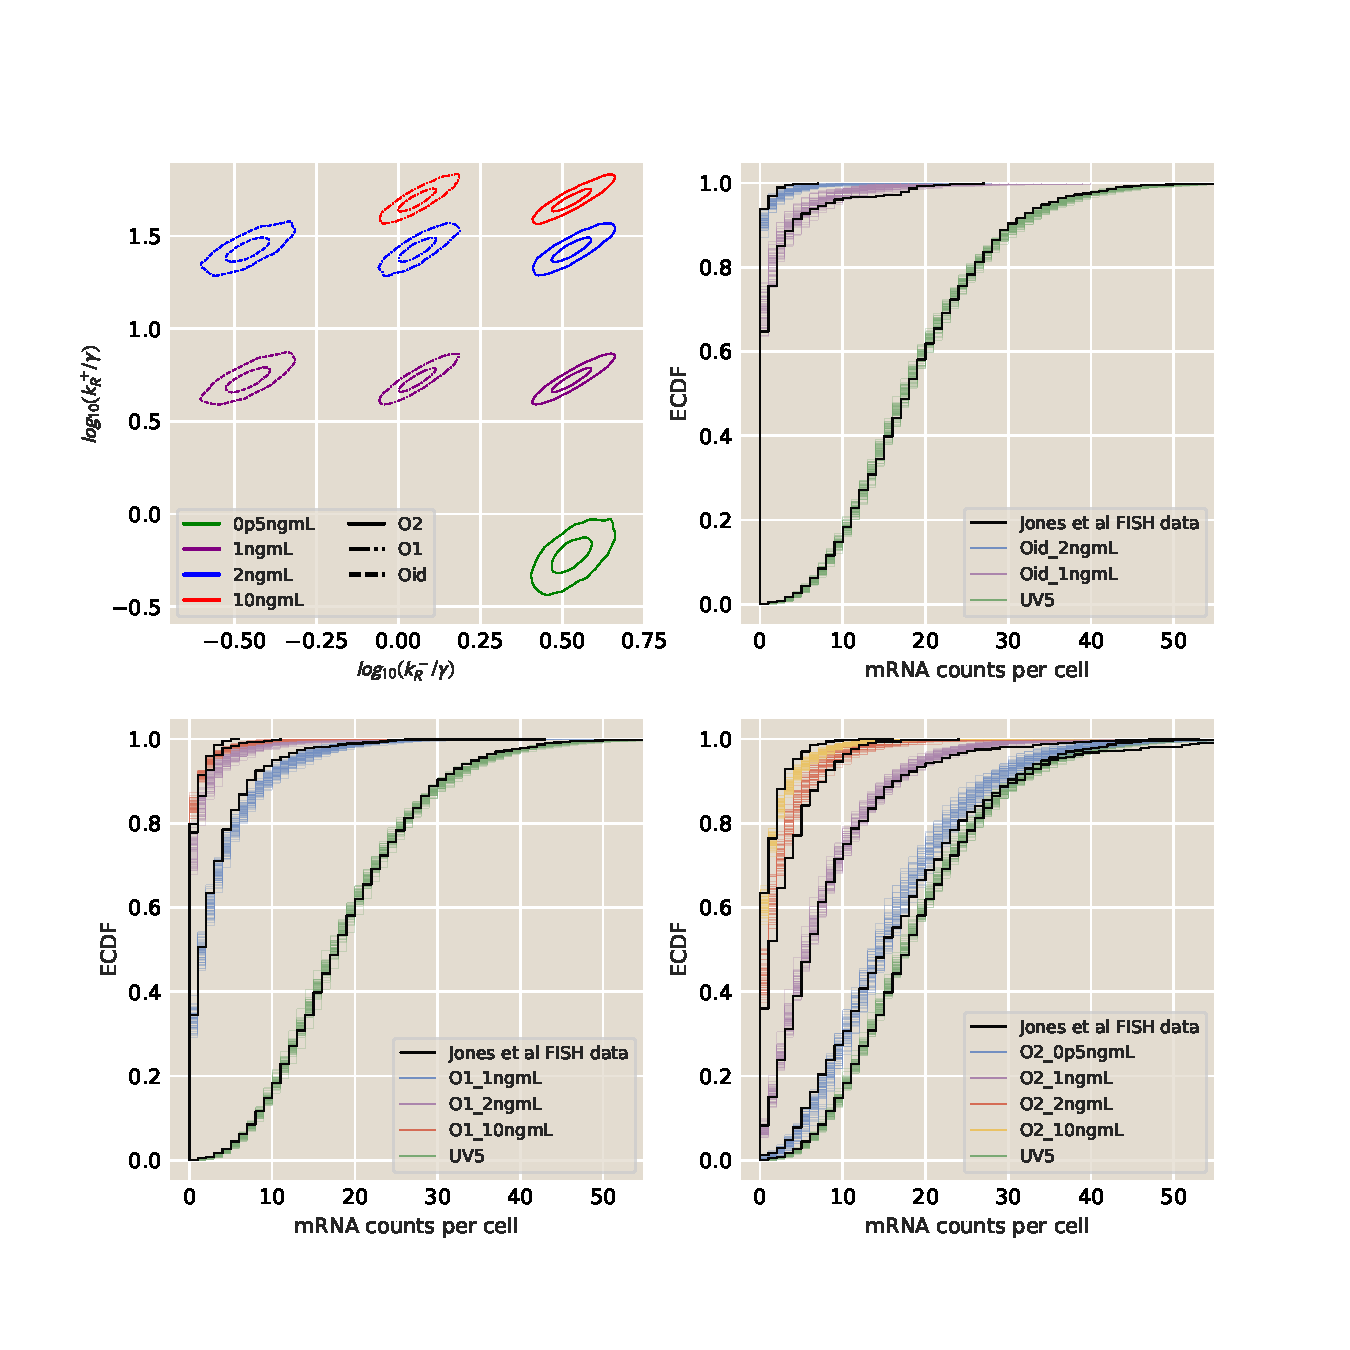
\includegraphics[width=0.9\textwidth]{../figures/figSIxx/ppc_many_pooled.pdf}
\caption{\textbf{Posterior predictive checks.}
(A) duplicates the posterior from~\fig{fig3:kR_inferences}B.
(B), (C), and (D) show samples from the posterior predictive distribution
for each of the datasets used in the inference.
Samples are sorted by operator and plotted separately simply for visual clarity.
The unrepressed promoter, UV5, is shown with each as a reference point.
\mmnote{
Obviously the PPC is not perfect,
but considering the relative simplicity of the model, I'm pleasantly surprised
how well it worked and that the model was even identifiable at all.
Interestingly, and perhaps not surprisingly, only 3 of the 9 datasets
were identifiable if fit in isolation: otherwise,
it was only by making assumptions that certain rates are equal
across datasets was identifiability achieved.
}
    }
\label{fig4:ppc}
\end{figure}

\appendix

\section{Derivations of constitutive promoter models}
\subsection{Model 2}
\mmnote{Obtain Fano factor from CME.}
\subsection{Model 3}
\mmnote{Obtain Fano factor by taking limit from Mitarai et al's expression.}
\subsection{Model 4}
\mmnote{Obtain Fano factor by relabeling cartoon from Jones2014.}

\section{Generating function solution for bursty promoters}

\subsection{Constitutive promoter with bursts}

\subsubsection{From master equation to generating function}

We would like to derive the full probability distribution of
mRNA copy number per cell for a model combining simple repression
with a promoter featuring bursty transcription initiation.
Before tackling mRNA and repression together, let us
just consider the bursty consititutive promoter,
model 4 in~\fig{fig:constit_post}
\mmnote{replicating Charlotte's notes; she says it's worked out
in~\cite{Paulsson2000}, but I don't see it, at least not in notation I can
comprehend. Need to find a cite for this,
or maybe just cite Charlotte, personal comm, since that's where I actually got it\dots}.
The master equation of interest is
\begin{align}
\deriv{t}p(m,t) = (m+1)\gamma p(m+1,t) - m\gamma p(m,t) - r p(m,t)
        + r \sum_{m^\prime=0}^m G_{m-m^\prime}(\theta) p(m^\prime,t),
\label{eq:1state_unreg_003}
\end{align}
where $G_{k}(\theta)$ is the geometric distribution defined as
\begin{align}
G_{k}(\theta) = \theta(1 - \theta)^k, \, k\in\{0,1,2,\dots\}.
\end{align}
With this convention, the mean burst size $b = (1-\theta)/\theta$.
$\gamma$ and $r$ are mRNA degradation rates and transcription burst
initiation rates, resp. The last term represents all ways the system could
end up with $m$ mRNAs, having started the burst with $m^\prime$. Define
$\lambda = r/\gamma$ and nondimensionalize time by $\gamma$, giving
\begin{align}
\deriv{t}p(m,t) = (m+1)p(m+1,t) - m p(m,t) - \lambda p(m,t)
        + \lambda \sum_{m^\prime=0}^m G_{m-m^\prime}(\theta) p(m^\prime,t),
\end{align}
The probability generating function is defined as
\begin{align}
F(z,t) = \sum_{m=0}^\infty z^m p(m,t).
\end{align}
Multiply both sides of the CME by $z^m$ and sum over all $m$ to get
\begin{align}
\pderiv[F]{t} = \sum_{m=0}^\infty z^m
\left(
(m+1)p(m+1,t) - m p(m,t) - \lambda p(m,t)
+ \lambda \sum_{m^\prime=0}^m G_{m-m^\prime}(\theta) p(m^\prime,t)
\right).
\end{align}
The first two terms can be rewritten as derivatives of the
generating function, i.e.,
\begin{align}
\sum_{m=0}^\infty z^m (m+1)p(m+1,t)
=
\pderiv{z} \sum_{m=0}^\infty z^{m+1} p(m+1,t)
=
\pderiv[F]{z}
\end{align}
and
\begin{align}
\sum_{m=0}^\infty z^m mp(m,t)
=
z\pderiv{z} \sum_{m=0}^\infty z^m p(m,t)
=
z\pderiv[F]{z}.
\end{align}
The final term is the most trouble. The trick is to reverse
the default order of the sums, as in
\begin{align}
&\lambda \sum_{m=0}^\infty \sum_{m^\prime=0}^m
        z^m \theta(1 - \theta)^{m-m^\prime} p(m^\prime,t)
\\=
&\lambda\theta \sum_{m^\prime=0}^\infty z^{m^\prime} p(m^\prime,t)
        \sum_{m=m^\prime}^\infty
        z^{m-m^\prime} (1 - \theta)^{m-m^\prime}
\\=
&\frac{\lambda\theta F}{1 - (1 - \theta)z}.
\end{align}
This works because after reordering the sums, the sum on $m$ is just
a geometric series. Its result is independent of $m^\prime$, so the sum on
$m^\prime$ reduces to the definition of the generating function.
Putting these results together, the PDE for the generation function is
\begin{align}
\pderiv[F]{t} = \pderiv[F]{z} - z\pderiv[F]{z} - \lambda F
        + \frac{\lambda\theta F}{1-z(1-\theta)}.
\end{align}
Changing variables to $\xi=1-\theta$ and simplifying gives
\begin{align}
\pderiv[F]{t} + (z - 1) \pderiv[F]{z} = \frac{(z-1)\xi}{1-z\xi}\lambda F.
\label{eq:1state_unreg_015}
\end{align}
\subsubsection{Stead-state}
At steady-state, the PDE reduces to the ODE
\begin{align}
\deriv[F]{z} = \frac{\xi}{1-z\xi}\lambda F,
\end{align}
which we can integrate as
\begin{align}
\int \frac{dF}{F} = \int \frac{\lambda\xi dz}{1-\xi z}.
\end{align}
The initial conditions for generating functions can be subtle and confusing.
The key fact follows from the definition
$F(z,t) = \sum_m z^m p(m,t)$,
normalization requires that
$F(z=1^-,t) = \sum_m p(m,t) = 1$.\footnote{
Sometimes the generating function may be undefined \textit{at} $z=1$ but the
limit still holds. Also many authors change variables from $z$ to other
things, so one must keep track of how the normalization condition transforms.
}
Doing the integrals (and producing constant $c$) gives
\begin{align}
\ln F &= -\lambda \ln(1-\xi z) + c
\\
F &= \frac{c}{(1-\xi z)^\lambda}.
\end{align}
Only one choice for $c$ can satisfy initial conditions, producing
\begin{align}
F(z) = \left(\frac{1-\xi}{1-\xi z}\right)^\lambda
        = \left(\frac{\theta}{1 - z(1-\theta)}\right)^\lambda,
\end{align}
which is exactly the negative binomial's generating function, as expected.

\subsection{Adding repression}
\subsubsection{Deriving the generating function for mRNA distribution}

Let us move from a one-state promoter to a two-state promoter, where one state
has repressor bound and the other produces transcriptional bursts as above.
A schematic of this model is shown in~\fig{fig3:kR_inferences}.
Although now we have an equation for each promoter state, otherwise
the master equation reads similarly to the one-state case, except with
additional terms corresponding to transitions between promoter states, namely
\begin{align}
\deriv{t}p_R(m,t) =& k_R^+ p_A(m,t) - k_R^- p_R(m,t)
        + (m+1)\gamma p_R(m+1,t) - m\gamma p_R(m,t)
\\
\begin{split}
\deriv{t}p_A(m,t) =& - k_R^+ p_A(m,t) + k_R^- p_R(m,t)
        + (m+1)\gamma p_A(m+1,t) - m\gamma p_A(m,t) 
\\
&- k_i p_A(m,t) + k_i \sum_{m^\prime=0}^m \theta(1-\theta)^{m-m^\prime} p_A(m^\prime,t),
\end{split}
\end{align}
where $p_R(m,t)$ is the probability of the system having $m$ mRNA copies
and having repressor bound to the promoter at time $t$, and $p_A$ is an
analogous probability to find the promoter without repressor bound.
$k_R+$ and $k_R^-$ are, respectively, the rates at which repressors
bind and unbind to and from the promoter, and
$\gamma$ is the mRNA degradation rate.
$k_i$ is the rate at which bursts initiate, and as before,
the geometric distribution of burst sizes has mean $b=(1-\theta)/\theta$.\footnote{
$\theta$ can be viewed as a Bernoulli trial probability: after each transcript
in a burst is produced, $\theta$ is the probability that the burst
terminates and $(1-\theta)$ is the probability that the burst continues.
}

Interestingly, it turns out that this problem maps exactly onto the
three-stage promoter model considered by
Shahrezaei and Swain in~\cite{Shahrezaei2008}, with relabelings.
Their approximate solution for protein distributions amounts to
the same approximation we make here in regarding the duration
of mRNA synthesis bursts as instantaneous, so their solution
for protein distributions also solves our problem of mRNA distributions.
Let us examine the analogy more closely.
They consider a two-state promoter, as we do here, but they model
mRNA as being produced one at a time and degraded, with rates
$v_0$ and $d_0$.
Then they model translation as occuring with rate $v_1$,
and protein degradation with rate $d_1$.
Now consider the limit where $v_1, d_0\rightarrow\infty$ with
their ratio $v_1/d_0$ held constant.
$v_1/d_0$ resembles the average burst size of translation from a single
mRNA: these are the rates of two Poisson processes that compete over a
transcript, which matches the story of geometrically distributed burst sizes.
So after taking this limit, on timescales slow compared to $v_1$ and $d_0$,
it appears that transcription events fire at rate $v_0$ and produce a
geometrically distributed burst of translation of mean size $v_1/d_0$,
which intuitively matches the story we have told above for mRNA
with variables relabeled.

To verify this intuitively conjectured mapping between our problem and
the solution in~\cite{Shahrezaei2008}, we continue with a careful
solution for the mRNA distribution using probability generating functions,
following the ideas sketched in~\cite{Shahrezaei2008}.
It is natural to nondimensionalize rates in the problem by $\gamma$,
or equivalently, this amounts to measuring time in units of $\gamma^{-1}$.
We are also only interested in steady state, so we set the time
derivatives to zero, giving
\begin{align}
0 =& k_R^+ p_A(m) - k_R^- p_R(m) + (m+1) p_R(m+1) - m p_R(m)
\\
\begin{split}
0 =& - k_R^+ p_A(m) + k_R^- p_R(m) + (m+1) p_A(m+1) - m p_A(m) 
\\
&- k_i p_A(m) + k_i \sum_{m^\prime=0}^m \theta(1-\theta)^{m-m^\prime} p_A(m^\prime),
\end{split}
\end{align}
        
The probability generating function is defined as before in the
constitutive case, except now we must introduce a generating function
for each promoter state,
\begin{align}
f_A(z) = \sum_{m=0}^\infty z^m p_A(m),
\;
f_R(z) = \sum_{m=0}^\infty z^m p_R(m).
\end{align}
Our real objective is the generating function $f(z)$ that generates
the mRNA distribution $p(m)$, independent of what state the promoter is in.
But since $p(m) = p_A(m) + p_R(m)$, it follows too that $f(z) = f_A(z) + f_R(z)$.

So as before we multiply both equations by $z^m$ and sum over all $m$.
Each individual term transforms exactly as did an analogous term in
the constitutive case, so the coupled ODEs for the generating functions read
\begin{align}
0 =& k_R^+ f_A(z) - k_R^- f_R(z) + \pderiv{z} f_R(z) - z \pderiv{z} f_R(z)
\\
\begin{split}
0 =&  - k_R^+ f_A(z) + k_R^- f_R(z) + \pderiv{z} f_A(z) - z \pderiv{z} f_A(z)
\\
&- k_i f_A(z) + k_i \frac{\theta}{1-z(1-\theta)} f_A(z),
\end{split}
\end{align}
and after changing variables $\xi = 1 - \theta$ as before
and rearranging, we have
\begin{align}
0 &= k_R^+ f_A(z) - k_R^- f_R(z) + (1-z) \pderiv{z} f_R(z)
\\
0 &=  - k_R^+ f_A(z) + k_R^- f_R(z) + (1 - z) \pderiv{z} f_A(z)
+ k_i \frac{(z-1)\xi}{1-z\xi} f_A(z),
\end{align}
We can transform this problem from two coupled first-order ODEs to a
single second-order ODE by solving for $f_A$ in the first and plugging
into the second, giving
\begin{align}
\begin{split}
0 = (1&-z) \pderiv[f_R]{z}
+ \frac{1-z}{k_R^+}
        \left(k_R^- \pderiv[f_R]{z} + \pderiv[f_R]{z} +(z-1) \psecderiv[f_R]{z}\right)
\\
&+ \frac{k_i}{k_R^+} \frac{(z-1)\xi}{1-z\xi}
        \left(k_R^- f_R + (z-1) \pderiv[f_R]{z}\right),
\end{split}
\end{align}
where, to reduce notational clutter, we have dropped the explicit $z$
dependence of $f_A$ and $f_R$. Simplifying we have
\begin{align}
0 = \psecderiv[f_R]{z}
        - \left(\frac{k_i\xi}{1-z\xi}
                + \frac{1 + k_R^- + k_R^+}{1-z}
        \right)\pderiv[f_R]{z}
        + \frac{k_i k_R^- \xi}{(1-z\xi)(1-z)}f_R.
\end{align}
This can be recognized as the hypergeometric differential equation,
with singularities at $z=1$, $z=\xi^{-1}$, and $z=\infty$. The latter
can be verified by a change of variables from $z$ to $x=1/z$,
being careful with the chain rule, and noting that $z=\infty$ is a
singular point if and only if $x=1/z=0$ is a singular point.

The standard form of the hypergeometric differential equation has its
singularities at 0, 1, and $\infty$, so to take advantage of the
standard form solutions to this ODE, we first need to transform
variables to put it into a standard form.
However, this is subtle. While any such transformation should work in
principle, the solutions are expressed most simply in the neighborhood
of $z=0$, but the normalization condition that we need to enforce
corresponds to $z=1$. The easiest path, therefore, is to find a change
of variables that maps
1 to 0, $\infty$ to $\infty$, and $\xi^{-1}$ to 1.
This is most intuitively done in two steps.

First map the $z=1$ singularity to 0 by the change of variables $v=z-1$, giving
\begin{align}
0 = \psecderiv[f_R]{v}
        + \left(\frac{k_i\xi}{(1+v)\xi - 1}
                + \frac{1 + k_R^- + k_R^+}{v}
        \right)\pderiv[f_R]{v}
        + \frac{k_i k_R^- \xi}{((1+v)\xi - 1)v}f_R.
\end{align}
Now two singularities are at $v=0$ and $v=\infty$.
The third is determined by $(1+v)\xi -1 = 0$, or $v=\xi^{-1} - 1$.
We want another variable change that maps this third singularity to 1
(without moving 0 or infinity). Changing variables again to
$w=\frac{v}{\xi^{-1} - 1} = \frac{\xi}{1-\xi} v$ fits the bill.
In other words, the combined change of variables
\begin{align}
w = \frac{\xi}{1-\xi} (z-1)
\end{align}
maps $z = \{1, \xi^{-1}, \infty\}$ to $w =\{0, 1, \infty\}$ as desired.
Plugging in, being mindful of the chain rule and noting
$(1 + v)\xi - 1 = (1 - \xi)(w - 1)$ gives
\begin{align}
0 = \left(\frac{\xi}{1-\xi}\right)^2 \psecderiv[f_R]{w}
+ \left(
        \frac{\xi k_i}{(1-\xi)(w-1)} + \frac{\xi(1 + k_R^- + k_R^+)}{(1-\xi)w}
\right) \frac{\xi}{1-\xi} \pderiv[f_R]{w}
+ \frac{k_i k_R^- \xi^2}{(1-\xi)^2 w(w-1)}f_R.
\end{align}
This is close to the standard form of the hypergeometric differential
equation, and some cancellation and rearrangement gives
\begin{align}
0 = w(w-1)\psecderiv[f_R]{w}
+ \left(k_i w + (1 + k_R^- + k_R^+)(w-1)\right) \pderiv[f_R]{w}
+ k_i k_R^- f_R.
\end{align}
and a little more algebra produces
\begin{align}
0 = w(1-w)\psecderiv[f_R]{w}
+ \left(1 + k_R^- + k_R^+
        - (1 + k_i + k_R^- + k_R^+)w
\right) \pderiv[f_R]{w}
- k_i k_R^- f_R,
\end{align}
which is the standard form. From this we can read off the solution
in terms of hypergeometric functions ${_2F_1}$ from
any standard source, e.g.~\cite{Abramowitz1964}, and identify the
conventional parameters in terms of our model parameters.
We want the general solution in the neighborhood of $w=0$ ($z=1$),
which for a homogeneous linear second order ODE must be a sum of two
linearly independent solutions.
More precisely,
\begin{align}
f_R(w) = C_1 {_2F_1}(\alpha, \beta, \gamma; w)
+ C_2 w^{1-\gamma}{_2F_1}(1+\alpha-\gamma, 1+\beta-\gamma, 2-\gamma; w)
\end{align}
with parameters determined by
\begin{align}
\begin{split}
\alpha\beta &= k_i k_R^-
\\
1+\alpha+\beta &= 1+k_i+k_R^-+k_R^+
\\
\gamma &= 1 + k_R^- + k_R^+
\end{split}
\end{align}
and constants $C_1$ and $C_2$ to be set by boundary conditions.
Solving for $\alpha$ and $\beta$, we find\footnote{
Note that $\alpha$ and $\beta$ are interchangeable in the definition of
${_2F_1}$ and differ only in the sign preceeding the radical.
}
\begin{align}
\begin{split}
\alpha &= \frac{1}{2}
\left(k_i+k_R^-+k_R^+ + \sqrt{(k_i+k_R^-+k_R^+)^2 - 4k_i k_R^-}\right)
\\
\beta &= \frac{1}{2}
\left(k_i+k_R^-+k_R^+ - \sqrt{(k_i+k_R^-+k_R^+)^2 - 4k_i k_R^-}\right)
\\
\gamma &= 1 + k_R^- + k_R^+.
\end{split}
\end{align}
Since the normalization condition requires that $f_R$ be finite at $w=0$,
we can immediately set $C_2=0$ to discard the second solution.
This is because all the rate constants are strictly positive,
so $\gamma>1$ and therefore $w^{1-\gamma}$ blows up as $w\rightarrow0$.
Now that we have $f_R$, we would like to find the generating function
for the mRNA distribution, $f(z) = f_A(z) + f_R(z)$.
We can recover $f_A$ from our solution for $f_R$, namely
\begin{align}
f_A(z) = \frac{1}{k_R^+}\left(k_R^- f_R(z) + (z-1) \pderiv[f_R]{z}\right)
\end{align}
or
\begin{align}
f_A(w) = \frac{1}{k_R^+}\left(k_R^- f_R(w) + w \pderiv[f_R]{w}\right),
\end{align}
where in the second line we transformed our original relation between
$f_R$ and $f_A$ to our new, more convenient, variable $w$.
Plugging our solution for $f_R(w) = C_1{_2F_1}(\alpha, \beta, \gamma; w)$
into $f_A$, we will require the differentiation rule for ${_2F_1}$,
which tells us
\begin{align}
\pderiv[f_R]{w} = C_1\frac{\alpha\beta}{\gamma}
                {_2F_1}(\alpha+1, \beta+1, \gamma+1; w),
\end{align}
from which it follows that
\begin{align}
f_A(w) = \frac{C_1}{k_R^+}
\left(
k_R^- {_2F_1}(\alpha, \beta, \gamma; w)
+ w\frac{\alpha\beta}{\gamma} {_2F_1}(\alpha+1, \beta+1, \gamma+1; w)
\right)
\end{align}
and therefore
\begin{align}
f(w) = C_1\left(1 + \frac{k_R^-}{k_R^+}\right)
        {_2F_1}(\alpha, \beta, \gamma; w)
+ w \frac{C_1}{k_R^+} \frac{\alpha\beta}{\gamma}
        {_2F_1}(\alpha+1, \beta+1, \gamma+1; w).
\end{align}
To proceed, we need one of the (many) useful identities known for
hypergeometric functions, in particular
\begin{align}
w\frac{\alpha\beta}{\gamma} {_2F_1}(\alpha+1, \beta+1, \gamma+1; w)
=
(\gamma-1)\left(
{_2F_1}(\alpha, \beta, \gamma-1; w) - {_2F_1}(\alpha, \beta, \gamma; w)
\right).
\end{align}
Substituting this for the second term in $f(w)$, we find
\begin{align}
f(w) = \frac{C_1}{k_R^+}
\left[
        \left(k_R^+ + k_R^-\right)
        {_2F_1}(\alpha, \beta, \gamma; w)
+ (\gamma-1)\left(
        {_2F_1}(\alpha, \beta, \gamma-1; w) - {_2F_1}(\alpha, \beta, \gamma; w)
        \right)
\right],
\end{align}
and since $\gamma-1 = k_R^+ + k_R^-$, the first and third terms cancel,
leaving only
\begin{align}
f(w) = C_1\frac{k_R^+ + k_R^-}{k_R^+} {_2F_1}(\alpha, \beta, \gamma-1; w).
\end{align}
Now we enforce normalization, demanding $f(w=0) = f(z=1) = 1$.
${_2F_1}(\alpha, \beta, \gamma-1; 0) = 1$, so we must have
$C_1 = k_R^+ / (k_R^+ + k_R^-)$ and consequently
\begin{align}
f(w) =  {_2F_1}(\alpha, \beta, k_R^+ + k_R^-; w).
\end{align}
Recalling that the mean burst size $b = (1-\theta)/\theta = \xi/(1-\xi)$
and $w = \frac{\xi}{1-\xi} (z-1) = b (z-1)$,
we can transform back to the original variable $z$ to find the tidy result
\begin{align}
f(z) =  {_2F_1}(\alpha, \beta, k_R^+ + k_R^-; b(z-1)),
\end{align}
with $\alpha$ and $\beta$ given above by
\begin{align}
\begin{split}
\alpha &= \frac{1}{2}
\left(k_i+k_R^-+k_R^+ + \sqrt{(k_i+k_R^-+k_R^+)^2 - 4k_i k_R^-}\right)
\\
\beta &= \frac{1}{2}
\left(k_i+k_R^-+k_R^+ - \sqrt{(k_i+k_R^-+k_R^+)^2 - 4k_i k_R^-}\right).
\end{split}
\end{align}
Finally we are in sight of the original goal. We can generate the
steady-state probability distribution of interest by
differentiating the generating function,
\begin{align}
p(m) = m! \left.\frac{\partial^m}{\partial z^m} f(z) \right|_{z=0},
\end{align}
which follows easily from its definition. Some contemplation reveals
that repeated application of the derivative rule used above will produce
products of the form $\alpha(\alpha+1)(\alpha+2)\cdots(\alpha+m-1)$ in
the expression for $p(m)$ and similarly for $\beta$ and $\gamma$. These
resemble ratios of factorials, but since $\alpha$, $\beta$, and $\gamma$
are not necessarily integer, we should express the ratios using gamma
functions instead. More precisely, one finds
\begin{align}
p(m) = \frac{
        \Gamma(\alpha + m)\Gamma(\beta + m)\Gamma(k_R^+ + k_R^-)
        }
        {
        \Gamma(\alpha)\Gamma(\beta)\Gamma(k_R^+ + k_R^- + m)
        }
\frac{b^m}{m!}{_2F_1}(\alpha+m, \beta+m, k_R^++k_R^-+m; -b)
\label{eq:p_m_bursty+rep}
\end{align}
which is finally the probability distribution we sought to derive.

\subsubsection{Moments}
We can verify the correctness of~\eq{eq:p_m_bursty+rep}
by comparison with Gillespie simulation.
We can also easily compute moments of the distribution from
the generating function, and check these against raw moments computed
directly from the master equation.

The $j$-th raw moment of the distribution can be computed from the
generating function from the formula
\begin{align}
\langle m^j \rangle
= \left. \left(z \frac{\partial}{\partial z}\right)^j f(z)\right|_{z=1}.
\end{align}
Note that \textit{probabilities} are generated by differentiating
and evaluating at $z=0$, while \textit{moments} are generated by
differentiating and evaluating at $z=1$. This also aligns with the
normalization constraint, which can be thought of as the zeroth raw moment.
        
The mean mRNA is given by
\begin{align}
\langle m \rangle = \left.z \pderiv[f]{z} \right|_{z=1}
= \frac{\alpha\beta b}{k_R^+ + k_R^-}
= k_i b\frac{k_R^-}{k_R^+ + k_R^-},
\end{align}
which is intuitive and appealingly simple:
the mean mRNA is just the mean mRNA in the absense of repression
($k_i b$, the burst rate time mean burst size)
times the fraction of time the repressor is bound, $k_R^-/(k_R^+ + k_R^-)$.

To compute the variance, let us first compute
\begin{align}
\begin{split}
\langle m^2\rangle
&= \left .z\pderiv{z}\left(z\pderiv[f]{z}\right) \right|_{z=1}
= \left. z\left(\pderiv[f]{z} + z\psecderiv[f]{z}\right)\right|_{z=1}
\\
&= \frac{\alpha\beta b}{k_R^+ + k_R^-}
        + \frac{\alpha(\alpha+1)\beta(\beta+1) b^2}
                {(k_R^+ + k_R^-)(k_R^+ + k_R^- + 1)}
\\
&= \frac{k_i b k_R^-}{k_R^+ + k_R^-}
        + \frac{k_i k_R^- b^2 (1 + k_i + k_R^+ + k_R^- + k_i k_R^-)}
                {(k_R^+ + k_R^-)(k_R^+ + k_R^- + 1)},
\end{split}
\end{align}
from which the variance is
\begin{align}
\begin{split}
var(m) = \langle m^2\rangle - \langle m\rangle^2
&= \frac{k_i b k_R^-}{k_R^+ + k_R^-}
\left(
1 + \frac{b(1 + k_i + k_R^+ + k_R^- + k_i k_R^-)} {k_R^+ + k_R^- + 1}
- \frac{k_i b k_R^-}{k_R^+ + k_R^-}
\right)
\\
&= k_i b\frac{k_R^-}{k_R^+ + k_R^-}
\left(
1 + b + k_i b\frac{1 + k_R^-} {k_R^+ + k_R^- + 1}
- \frac{k_i b k_R^-}{k_R^+ + k_R^-}
\right)
\\
&= k_i b\frac{k_R^-}{k_R^+ + k_R^-}
\left(
1 + b + k_i b\frac{k_R^+}{(k_R^+ + k_R^-)(k_R^+ + k_R^- + 1)}
\right).
\end{split}
\end{align}
The Fano factor is the quantity in parentheses. This can be interpreted as
the variability arising from the negative binomial distribution of the
unregulated promoter $(1+b)$ plus additional noise arising from repression.

\mmnote{Still to writeup: moment derivation direct from CME to compare}

\subsection{Numerical considerations and recursion formulas}
\subsubsection{Generalities}
We would like to carry out Bayesian parameter inference on FISH data
from~\cite{Jones2014}, using~\eq{eq:p_m_bursty+rep} as our
likelihood. This requires accurate (and preferably fast)
numerical evaluation of the hypergeometric function ${_2F_1}$,
which is a notoriously hard problem~\cite{Pearson2017, Gil2007},
and our particular needs here present an especial challenge as we show below.

The hypergeometric function is defined by its Taylor series as
\begin{align}
{_2F_1}(a,b,c;z) 
= \sum_{l=0}^\infty
\frac{\Gamma(a + l)\Gamma(b + l)\Gamma(c)}
        {\Gamma(a)\Gamma(b)\Gamma(c + l)}
\frac{z^l}{l!}
\end{align}
for $|z|<1$, and by analytic continuation elsewhere.
If $z\lesssim1/2$ and $\alpha$ and $\beta$ are not too large
(absolute value below 20 or 30),
then the series converges quickly and an accurate numerical representation is
easily computed by truncating the series after a reasonable number of terms.
Unfortunately, we need to evaluate ${_2F_1}$ over mRNA copy numbers fully out
to the tail of the distribution, which can easily reach 50, possibly 100.
From~\eq{eq:p_m_bursty+rep}, this means evaluating ${_2F_1}$
repeatedly for values of $a$, $b$, and $c$ spanning the full range
from $\mathcal{O}(1)$ to $\mathcal{O}(10^2)$,
even if $\alpha$, $\beta$, and $\gamma$
in~\eq{eq:p_m_bursty+rep} are small,
with the situation even worse if they are not small.
A naive numerical evaluation of the series definition will be
prone to overflow and, if any of $a,b,c<0$, then some successive terms in the
series have alternating signs which can lead to catastrophic cancellations.

One solution is to evaluate ${_2F_1}$ using arbitrary precision arithmetic
instead of floating point arithmetic,
e.g., using the \texttt{mpmath} library in Python.
This is accurate but incredibly slow computationally.
To quantify how slow, we found that
evaluating the likelihood defined by~\eq{eq:p_m_bursty+rep} $\sim50$ times
(for a typical dataset of interest from~\cite{Jones2014},
with $m$ values spanning 0 to $\sim50$)
using arbitrary precision arithmetic is 100-1000 fold slower than
evaluating a negative binomial likelihood for the corresponding
constitutive promoter dataset.

To claw back $\gtrsim30$ fold of that slowdown, we can exploit
one of the many catalogued symmetries involving ${_2F_1}$.
The solution involves recursion relations originally explored by Gauss,
and studied extensively in~\cite{Pearson2017, Gil2007}.
They are sometimes known as contiguous relations and relate the values
of any set of 3 hypergeometric functions whose arguments differ by integers.
To rephrase this symbolically, consider a set of hypergeometric functions
indexed by an integer $n$,
\begin{align}
f_n = {_2F_1}(a+\epsilon_i n, b+\epsilon_j n, c+\epsilon_k n; z),
\end{align}
for a fixed choice of $\epsilon_i, \epsilon_j, \epsilon_k \in \{0,\pm 1\}$
(at least one of $\epsilon_i, \epsilon_j, \epsilon_k$ must be nonzero,
else the set of $f_n$ would contain only a single element).
Then there exist known recurrence relations of the form
\begin{align}
A_n f_{n-1} + B_n f_{n} + C_n f_{n+1} = 0,
\end{align}
where $A_n, B_n$, and $C_n$ are some functions of $a,b,c$, and $z$.
In other words, for fixed $\epsilon_i, \epsilon_j, \epsilon_k, a, b,$ and $c$,
if we can merely evaluate ${_2F_1}$ twice, say for $n^\prime$ and $n^\prime-1$,
then we can easily and rapidly generate values for arbitrary $n$.

This provides a convenient solution for our problem: we need repeated
evaluations of ${_2F_1}(a+m, b+m, c+m; z)$
for fixed $a,b$, and $c$ and many integer values of $m$.
They idea is that we can use arbitrary precision arithmetic to evaluate
${_2F_1}$ for just two particular values of $m$ and then generate
${_2F_1}$ for the other 50-100 values of $m$ using the recurrence
relation.\footnote{
There are even more sophisticated ways of utilizing the recurrence
relations that might have netted another factor of 2 speed-up, and
possibly as much as a factor of 10, but the method described here had
already reduced the computation time to an acceptable
$\mathcal{O}(\text{1 min})$, so these more sophisticated approaches did
not seem worth the time to pursue.
}

However, there two further wrinkles.
The first is that
a naive application of the recurrence relation is numerically unstable.
Roughly, this is because the three term recurrence relations,
like second order ODEs, admit two linearly independent solutions.
In a certain eigenbasis, one of these solutions dominates the other
as $n\rightarrow\infty$, and as $n\rightarrow-\infty$,
the dominance is reversed.
If we fail to work in this eigenbasis, our solution of the recurrence relation
will be a mixture of these solutions and rapidly accumulate numerical error.
For our purposes, it suffices to know that the authors of~\cite{Gil2007}
derived the numerically stable solutions (so-called \textit{minimal solutions})
for several possible choices of $\epsilon_i, \epsilon_j, \epsilon_k$.
Running the recurrence in the proper direction using a minimal solution
is numerically robust and can be done entirely in floating point arithmetic, 
so that we only need to evaluate ${_2F_1}$ with arbitrary precision arithmetic
to generate the seed values for the recursion.

The second wrinkle is a corollary to the first.
The minimal solutions are only minimal for certain ranges of the argument $z$,
and not all of the 26 possible recurrence relations
have minimal solutions for all $z$.
This can be solved by using one of the many transformation formulae for
${_2F_1}$ to convert to a different recurrence relation that has
a minimal solution over the required domain of $z$, although
this can require some trial and error to find the right transformation,
the right recurrence relation, and the right minimal solution.

\subsubsection{Particulars}
Let us now demonstrate these generalities for our problem of interest.
In order to evaluate the probability distribution of our
model,~\eq{eq:p_m_bursty+rep}, we need to evaluate hypergeometric functions
of the form ${_2F_1}(\alpha+m, \beta+m, \gamma+m; -b)$
for values of $m$ ranging from $0$ to $\mathcal{O}(100)$.
The authors of~\cite{Gil2007} did not derive a recursion relation
for precisely this case. We could follow their methods and do so ourselves,
but it is much easier to convert to a case that they did consider.
The strategy is to look through the minimal solutions tabulated
in~\cite{Gil2007} and search for a transformation we could apply to
${_2F_1}(\alpha+m, \beta+m, \gamma+m; -b)$ that would place the $m$'s
(the variable being incremented by the recursion)
in the same arguments of ${_2F_1}$ as the minimal solution.
After some ``guess and check,'' we found that the transformation
\begin{align}
{_2F_1}(\alpha+m, \beta+m, \gamma+m; -b)
=
(1+b)^{-\alpha-m}
        {_2F_1}\left(\alpha+m, \gamma-\beta, \gamma+m; \frac{b}{1+b}\right),
\label{eq:rec_euler_pretransform}
\end{align}
produces a ${_2F_1}$ on the right hand side that closely resembles
the minimal solutions $y_{3,m}$ and $y_{4,m}$ in Eq.~4.3 in~\cite{Gil2007}.
Explicitly, these solutions are
\begin{align}
y_{3,m}
&\propto
{_2F_1}\left(-\alpha^\prime + \gamma^\prime - m,
                -\beta^\prime + \gamma^\prime,
                1-\alpha^\prime-\beta^\prime+\gamma^\prime-m;
                1-z\right)
\\
y_{4,m}
&\propto
{_2F_1}\left(\alpha^\prime + m,
                \beta^\prime,
                1+\alpha^\prime+\beta^\prime-\gamma^\prime+m;
                1-z\right),
\label{eq:minimal_soln_sans_prefac}
\end{align}
where we have omitted prefactors which are unimportant for now.
Which of these two we should use depends on what values $z$ takes on.
Equating $1-z=b/(1+b)$ gives $z=1/(1+b)$, and since $b$ is strictly positive,
$z$ is bounded between 0 and 1.
From Eq.~4.5 in~\cite{Gil2007}, $y_{4,m}$ is the minimal solution
for real $z$ satisfying $0<z<2$, so this is the only minimal solution we need.

Now that we have our minimal solution,
what recurrence relation does it satisfy?
Confusingly, the recurrence relation of which $y_{4,m}$ is a solution
increments different arguments of ${_2F_1}$ that does $y_{4,m}$:
it increments the first only, rather than first and third.
This recurrence relation can be looked up, e.g., Eq.~15.2.10
in~\cite{Abramowitz1964}, which is
\begin{align}
(\gamma^\prime - (\alpha^\prime + m)) f_{m-1}
+
(2(\alpha^\prime+m) - \gamma^\prime + (\beta^\prime - \alpha^\prime)z)f_m
+ \alpha^\prime(z-1) f_{m+1} = 0.
\label{eq:chosen_rec_rel}
\end{align}
Now we must solve for the parameters appearing in the recurrence relation
in terms of our parameters, namely by setting
\begin{align}
\begin{split}
\alpha^\prime &= \alpha
\\
\beta^\prime &= \gamma - \beta
\\
1 + \alpha^\prime + \beta^\prime - \gamma^\prime &= \gamma
\\
1 - z &= \frac{b}{1+b}
\end{split}
\end{align}
and solving to find
\begin{align}
\begin{split}
\alpha^\prime &= \alpha
\\
\beta^\prime &= \gamma - \beta
\\
\gamma^\prime &= 1 + \alpha - \beta
\\
z &= \frac{1}{1+b}
.
\end{split}
\end{align}
Finally we have everything we need. The minimal solution
\begin{align}
y_{4,m}
=
\frac{\Gamma(1+\alpha^\prime-\gamma^\prime+m)}
        {\Gamma(1+\alpha^\prime+\beta^\prime-\gamma^\prime+m)}
\times
{_2F_1}\left(\alpha^\prime + m,
                \beta^\prime,
                1+\alpha^\prime+\beta^\prime-\gamma^\prime+m;
                1-z\right),
\end{align}
where we have now included the necessary prefactors,
is a numerically stable solution of the recurrence
relation~\eq{eq:chosen_rec_rel} if the recursion is run
from large $m$ to small $m$.
So the procedure is to compute the value of ${_2F_1}$ for the two
largest $m$ values of interest using arbitrary precision arithmetic,
compute the prefactors to construct
$y_{4,\text{max}(m)}$ and $y_{4,\text{max}(m)-1}$,
recursively compute $y_{4,m}$ for all $m$ less than $\text{max}(m)$ down
to $m=0$, then cancel off the prefactors of the resulting values of
$y_{4,m}$ for all $m$ to produce ${_2F_1}$ for all desired $m$ values.
\mmnote{Maybe I should reformat this paragraph into
a pseudocode version of the algorithm?
Instead of, or in addition to?}

With ${_2F_1}$ computed, the only remaining numerical danger in computing
$p(m)$ in~\eq{eq:p_m_bursty+rep} is overflow of the gamma functions.
This is easily solved by taking the log of the entire expression
and using standard routines to compute the log of the gamma functions,
then exponentiating the entire expression at the end if $p(m)$
is needed rather than $\log p(m)$.

%%%%%%%%%%%%%%%%%%%%% APPENDICES %%%%%%%%%%%%%%%%%%%%%%%%%%%%%%%%%%%
\appendix


% \bibliographystyle{nature}
\bibliographystyle{abbrv}
\bibliography{./library}

\end{document}
